\documentclass{beamer}
\usepackage[fontsize=20pt]{fontsize}
\usepackage{graphicx}
\usepackage{tikz}
\usepackage{svg}
\usepackage[polish]{babel}
\graphicspath{ {./images/} }
\usetheme{Warsaw}

%Information to be included in the title page:

% Custom title page layout adjustments
\title{\large Porównanie wydajności i możliwości współczesnych silników do gier komputerowych}
\author{Krzysztof Rudnicki}
\institute{
    \textbf{Promotor} \\
    dr inż. Michał Chwesiuk
}
\date{\scriptsize \today} % Adjust the font size here


\setbeamertemplate{footline}[frame number]{}
\beamertemplatenavigationsymbolsempty
\setbeamertemplate{headline}{}






\begin{document}

\begin{frame}
  \vspace{-0.5cm} % Adjust vertical space above title
  \maketitle
  % Alternatively, use a completely custom layout:
  %\begin{center}
  %    {\Large\inserttitle\par}
  %    \vskip1em
  %    {\insertauthor\par}
  %    \vskip1em
  %    {\insertinstitute\par}
  %    \vskip1em
  %    {\insertdate\par}
  %\end{center}
\end{frame}

\begin{frame}
\frametitle{Plan prezentacji}
\tableofcontents
\end{frame}

\section{Definicje}
\begin{frame}
  \frametitle{Gra komputerowa}
  \large Aplikacja dostępna na platformie "Steam" oznaczona typem "Game"
\end{frame}
\begin{frame}
\frametitle{Silnik do gier}
\large Oprogramowanie zaprojektowane i stworzone do kreacji gier komputerowych
\end{frame}

\begin{frame}
  \frametitle{Nowoczesne}
  \large Ponad 1000 gier w tej dekadzie na platformie "Steam"
\end{frame}


{
  \setbeamercolor{footline}{fg=white}
\usebackgroundtemplate{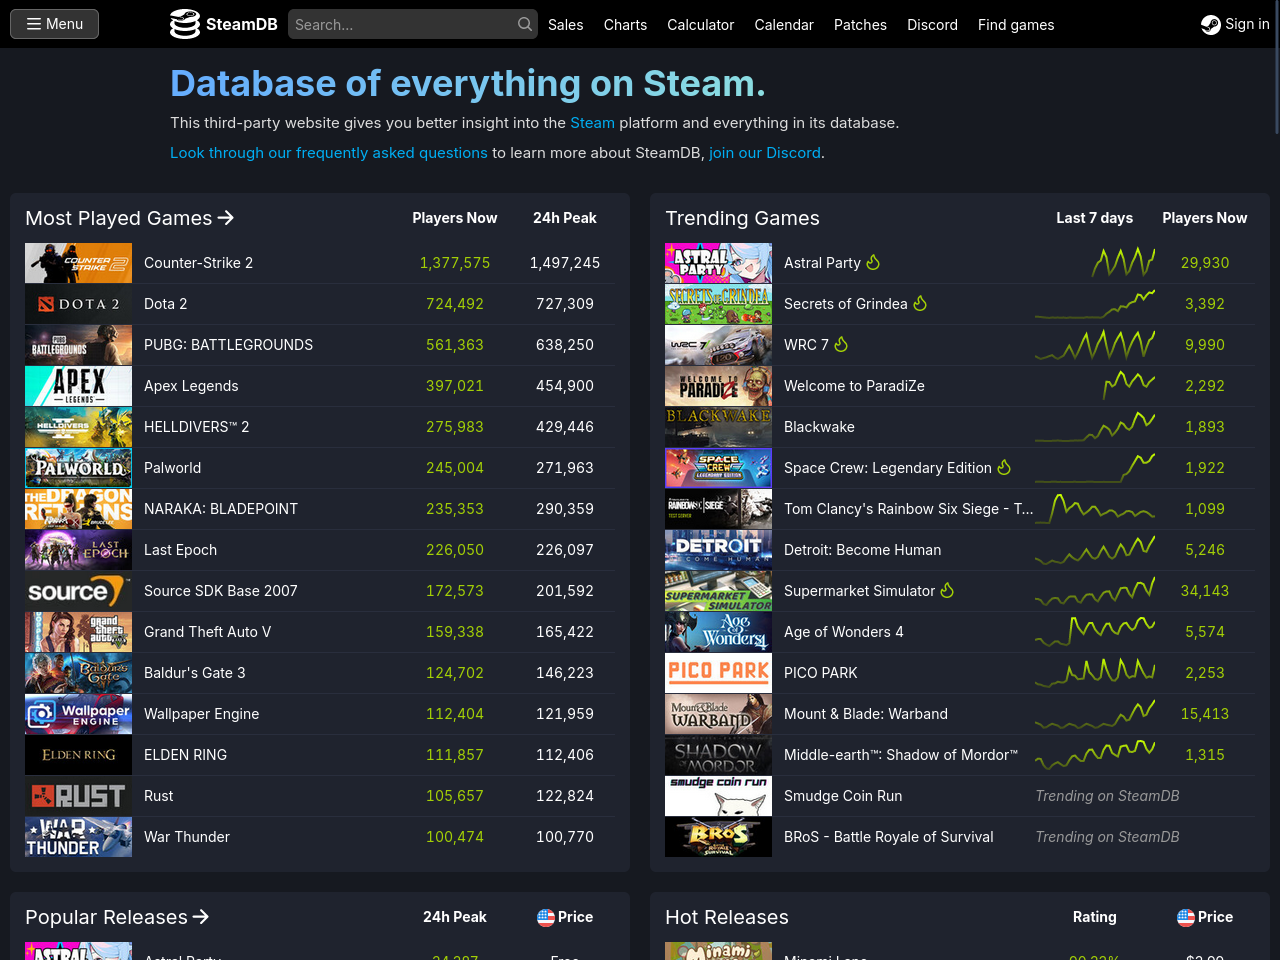
\includegraphics[width=\paperwidth, height=\paperheight]{steamdb_main.png}}
\begin{frame}
\end{frame}
}


{
\usebackgroundtemplate{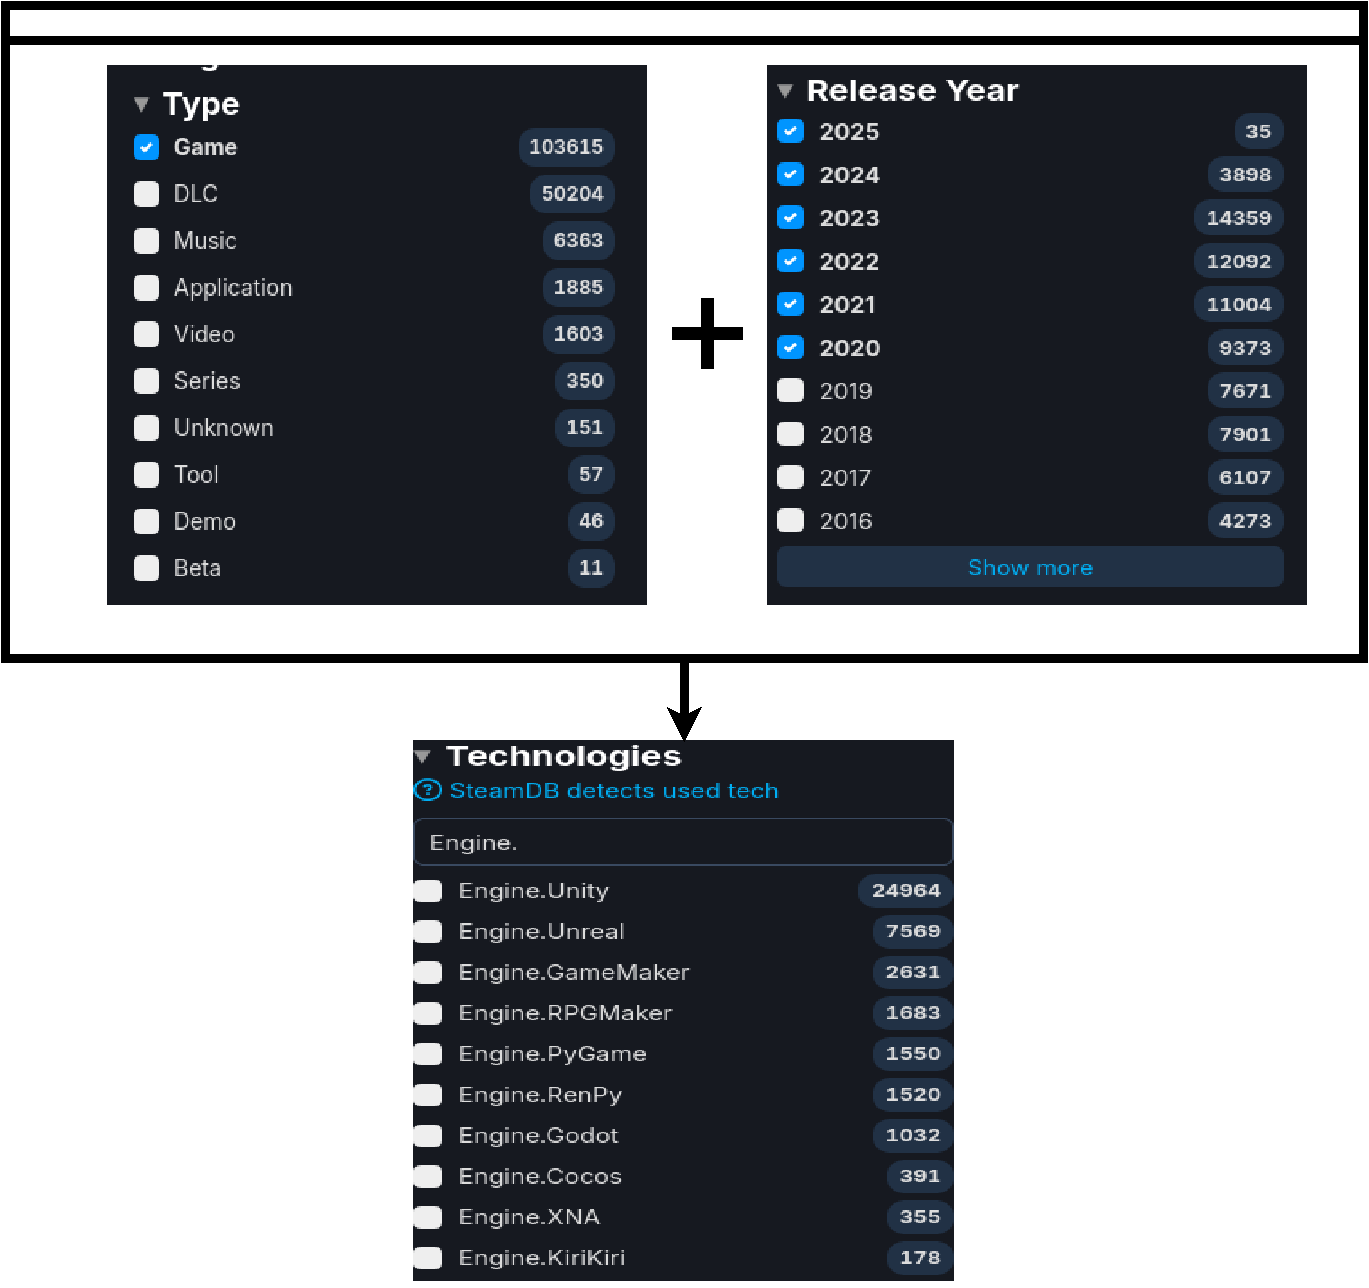
\includegraphics[width=\paperwidth, height=\paperheight]{steamdb_filter.drawio.pdf}}
\begin{frame}
\end{frame}
}

\begin{frame}
  \frametitle{Wybrane silniki}
  \begin{center}    
  
\includegraphics[width=0.8\paperwidth, height=0.8\paperheight]{usedEngines.pdf}
\end{center}
\end{frame}

\begin{frame} 
  \frametitle{Wydajność silnika}
  \begin{itemize}
    \item Klatki na sekundę (FPS)
    \item Zużycie CPU, GPU, RAM i VRAM
    \item Liczba draw calls 
    \item Czas ładowania assetów 
    \item Czas odpowiedzi na interakcję gracza
  \end{itemize} 
\end{frame}
\begin{frame}
    \frametitle{Możliwości Silnika}
    \begin{itemize}
        \item Renderowanie grafiki 
        % Ray tracing, HDR lighting, dynamic shadows, particle systems, animacja
        \item Silnik Fizyczny 
        \item Multiplatformowość (VR)
        % Linux, Windows, MacOS, Android, IOs, Xbox, PlayStation, Nintendo, VR
        \item Skryptowanie logiki gier (AI)
        \item Gry online
        \item Sklepy z assetami
    \end{itemize}
  \end{frame}
    \section{Narzędzia}
      \frametitle{Unity Profiler}
      {
        \setbeamercolor{footline}{fg=white}
        \usebackgroundtemplate{
          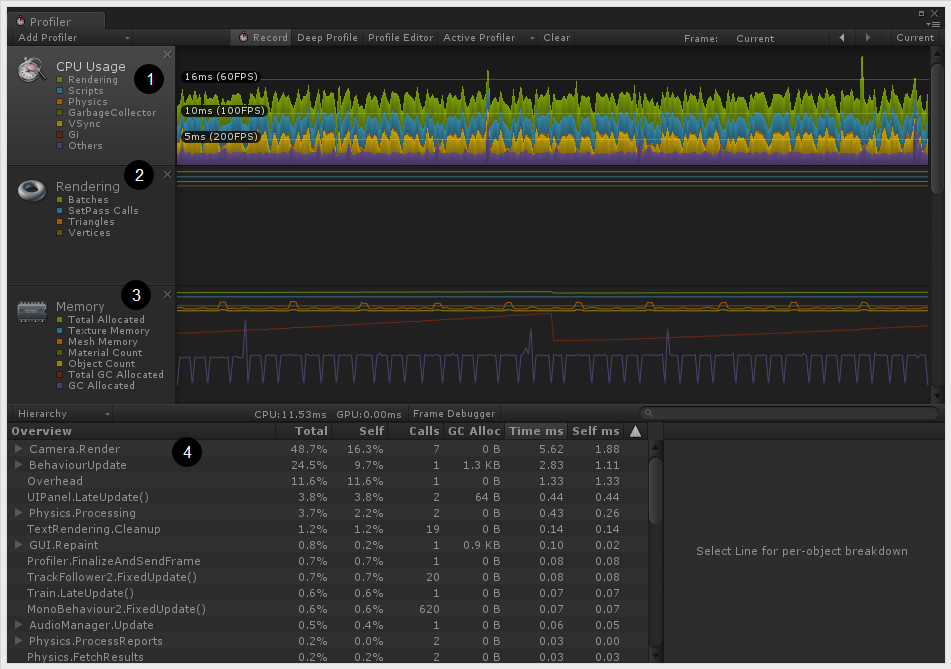
\includegraphics[width=\paperwidth, height=\paperheight]
          {unity_profiler.png}}
        \begin{frame}
        \end{frame}
        }

        \frametitle{Unreal Profiler}
        {
          \setbeamercolor{footline}{fg=white}
          \usebackgroundtemplate{
            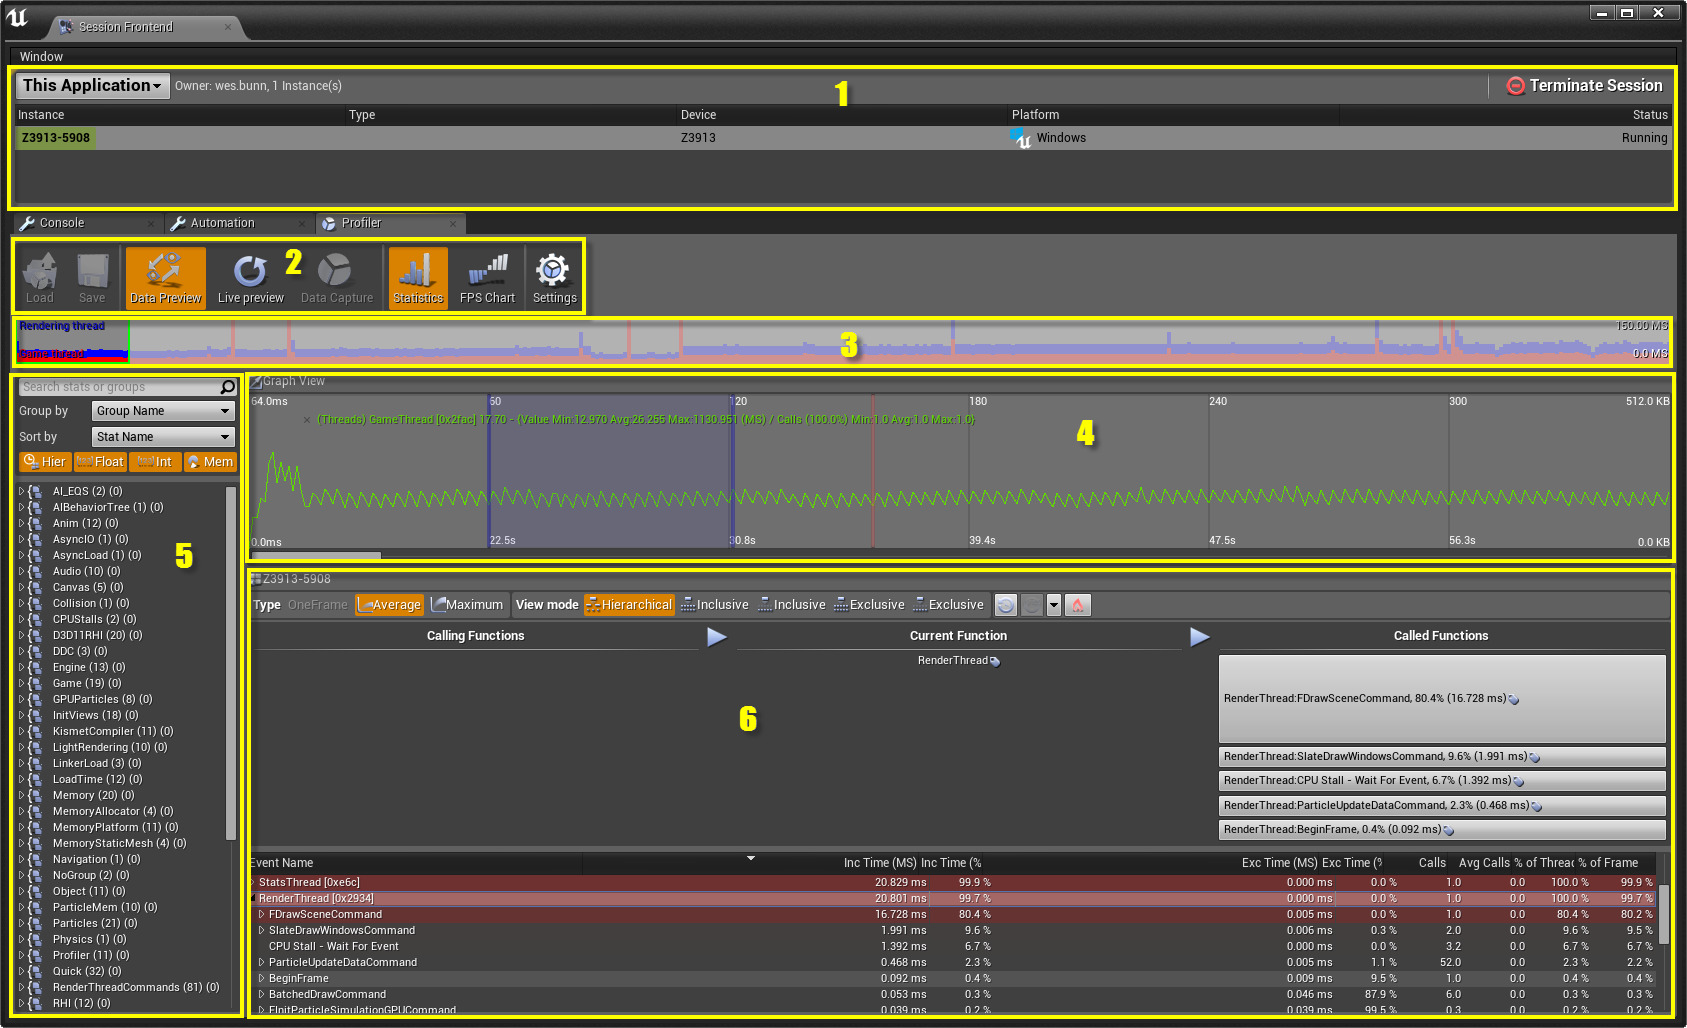
\includegraphics[width=\paperwidth, height=\paperheight]
            {unreal_profiler.jpg}}
          \begin{frame}
          \end{frame}
          }

          \frametitle{Nvida nsight}
          {
            \setbeamercolor{footline}{fg=white}
            \usebackgroundtemplate{
              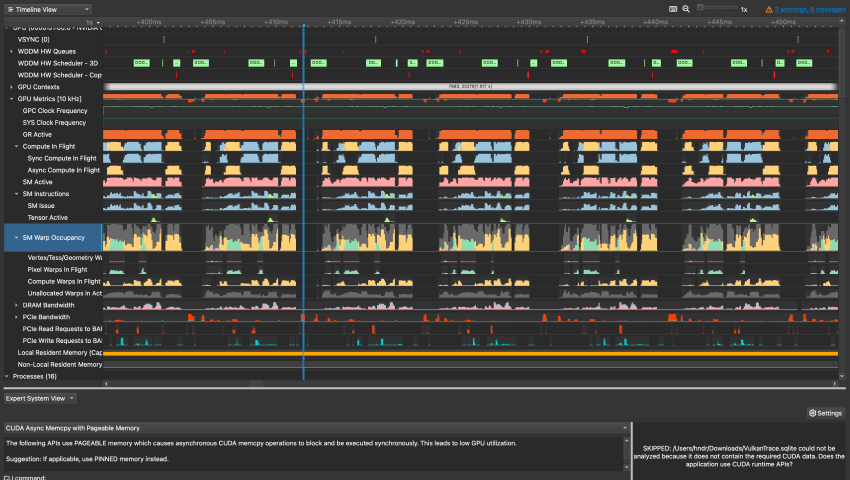
\includegraphics[width=\paperwidth, height=\paperheight]
              {nvida_nsighty.jpg}}
            \begin{frame}
            \end{frame}
            }
        
    \section{Podsumowanie}
\begin{frame}
    Thesis is about creating a game engine specialized in match-three multiplatform games using OpenGL
    \frametitle{Summary}
    \end{frame}

    \section{Źródła}
\begin{frame}
    \begin{itemize}
        \item \href{https://docs.gl/}{https://docs.gl/}
    \item \href{https://learnopengl.com/}{https://learnopengl.com/}
    \item \href{https://www.youtube.com/c/gameengineseries}{The Cherno}
    \item Game Engine Architecture, Jason Gregory
    \end{itemize}
    \frametitle{References/sources}
    \end{frame}

\end{document}